\chapter{Przerzutnik Schmidta}

\section{Budowa układu}

\begin{itemize}
    \item Do budowy układu wykorzystano oporniki \textbf{100}$\boldsymbol{\Omega}$ oraz \textbf{10k}$\boldsymbol{\Omega}$ znajdujących się na płytce, które pozwalają na dynamiczną zmianę oporu.
    \item Za pomocą trójnika doprowadzono sygnał zarówno do płytki, jak i do oscyloskopu.
        \begin{figure}[H]
            \centering
            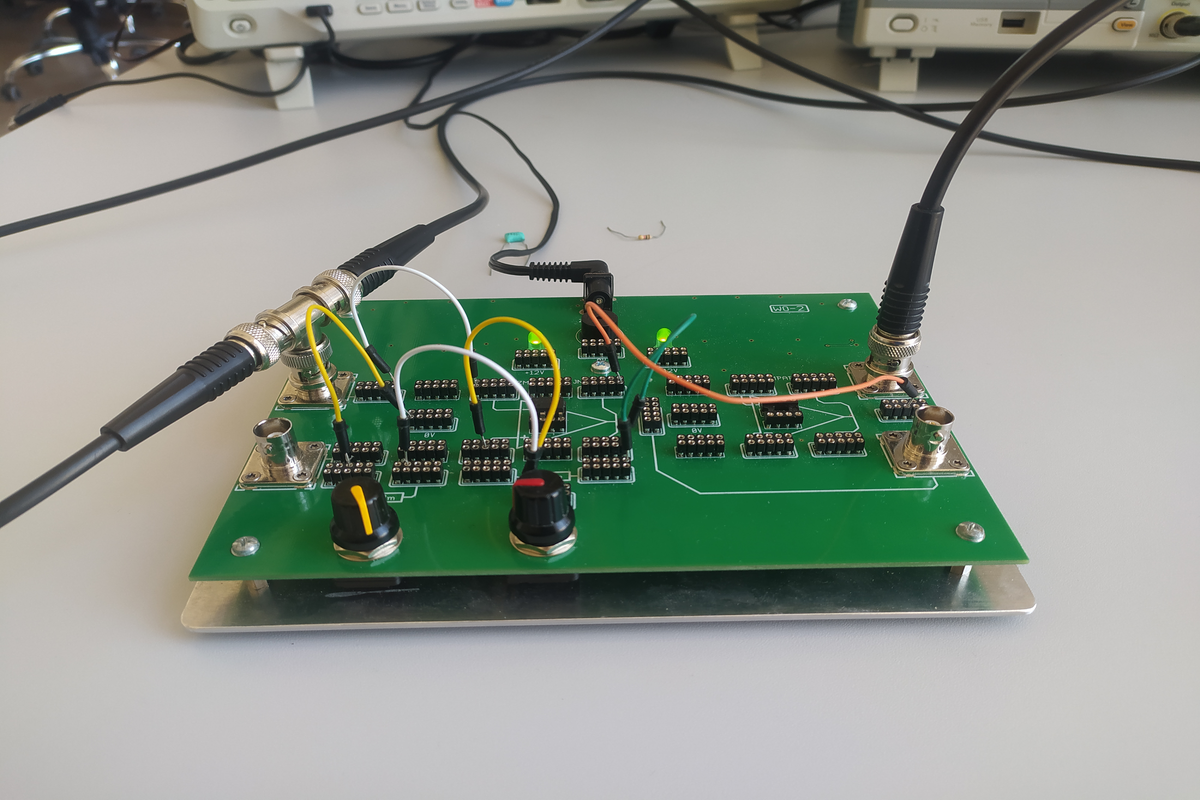
\includegraphics[scale=0.17]{img/phone/1651502036786_scaled.png}
            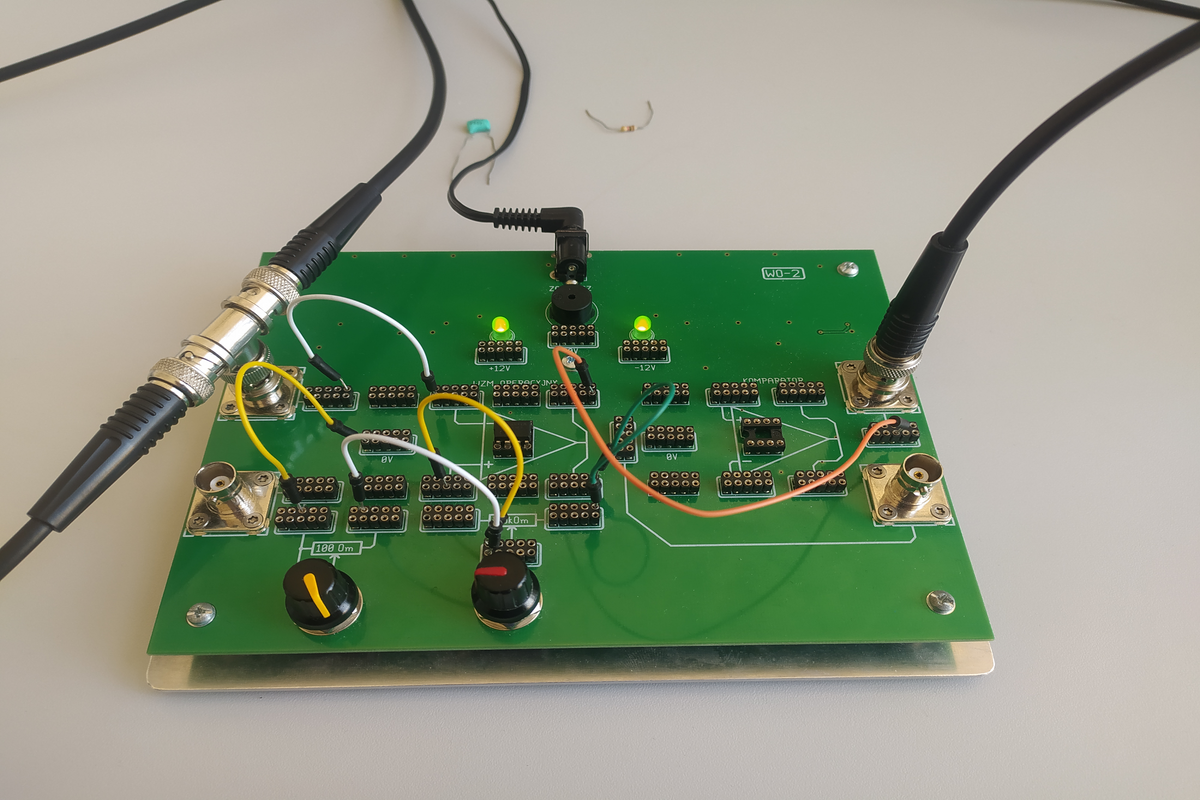
\includegraphics[scale=0.17]{img/phone/1651502036800_scaled.png}
            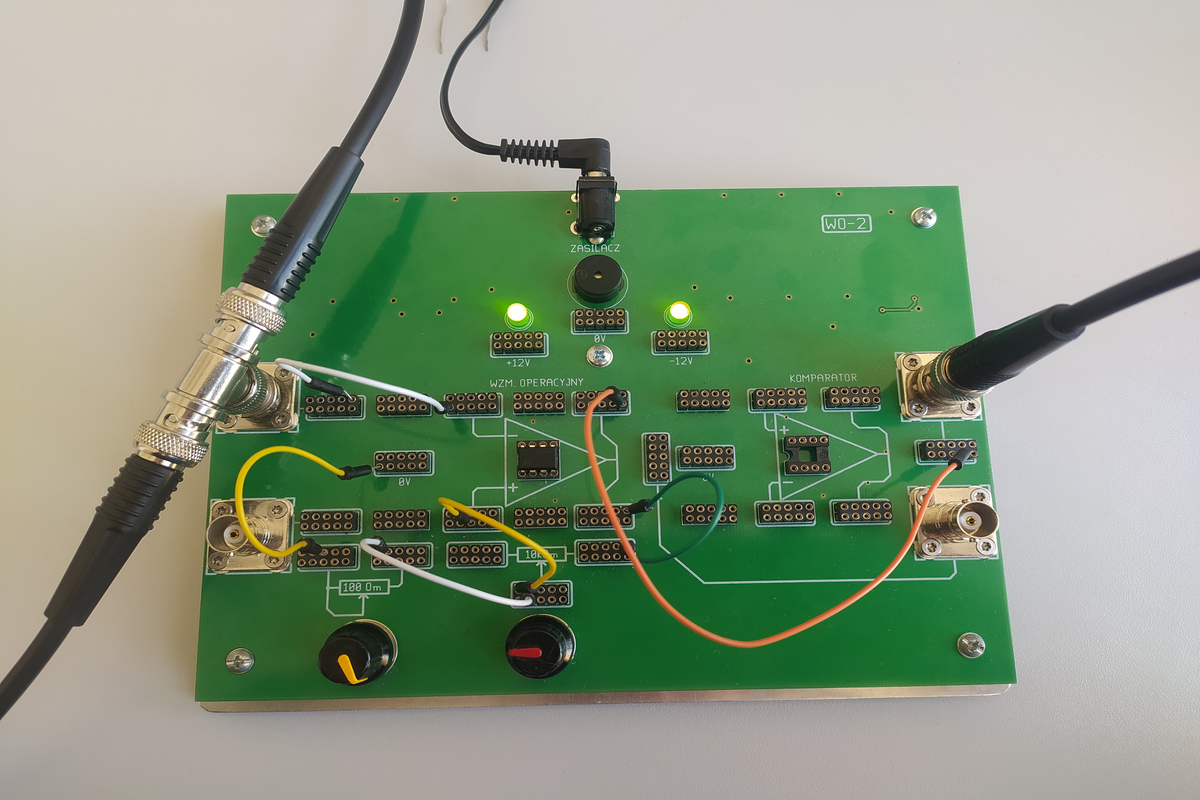
\includegraphics[scale=0.23]{img/phone/1651502036813_scaled.png}
            \caption{Zbudowany przerzutnik Schmidta}
            \label{fig:przerzutnik_schmidta}
        \end{figure}
\end{itemize}

\pagebreak

\section{Przebiegi napięcia wyjściowego}

\begin{itemize}
    \item Przebiegi zostały pobrane przy wartościach oporników równych:
        \begin{gather}
            \label{przerzutnik:R1} R_1 = \textbf{85.9}\boldsymbol{\Omega} \\
            \label{przerzutnik:R2} R_2 = \textbf{1k}\boldsymbol{\Omega}
        \end{gather}
    \item Przebieg napięcia wyjściowego gdy na wejściu podany został sygnał sinusoidalny oraz sygnał trójkątny (oba o wartościach \textbf{1V}, \textbf{1kHz}):
        \begin{figure}[H]
            \centering
            \begin{subfigure}[h]{0.49\textwidth}
                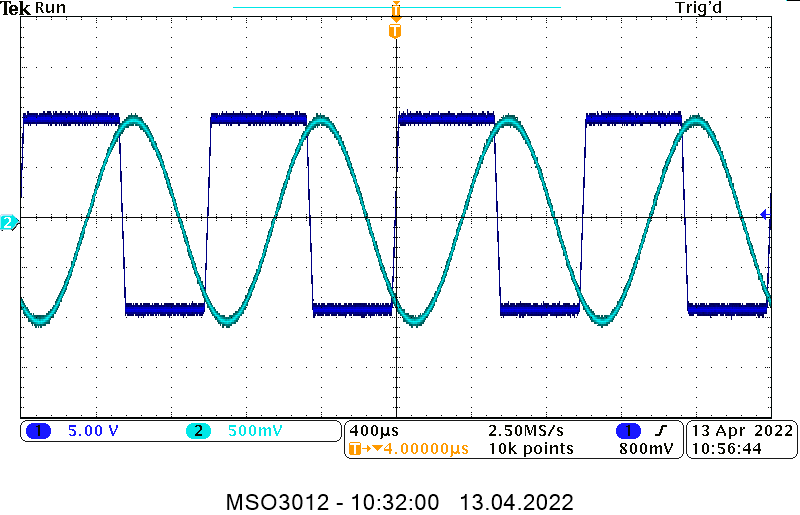
\includegraphics[width=\textwidth]{img/osciloscope/1_4_histereza_przeskok_sin_cropped.png}
                \caption*{Sygnał sinusoidalny}
            \end{subfigure}
            \begin{subfigure}[h]{0.49\textwidth}
                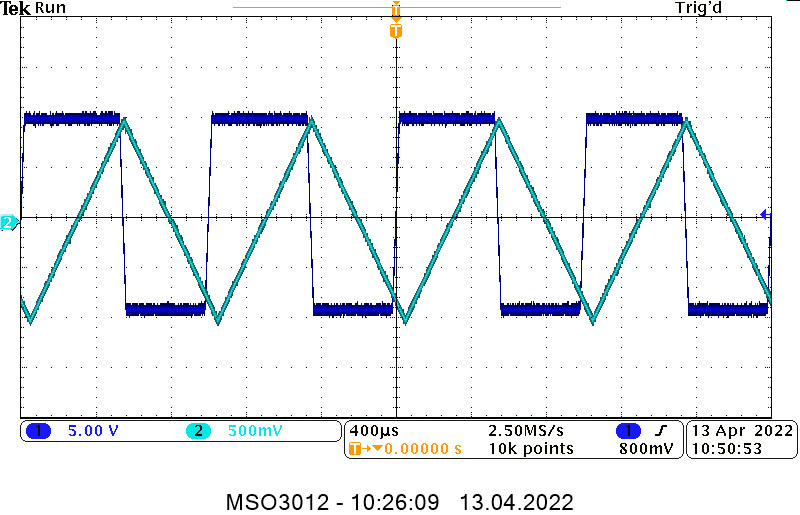
\includegraphics[width=\textwidth]{img/osciloscope/1_4_histereza_przeskok_trojkat_cropped.png}
                \caption*{Sygnał trójkątny}
            \end{subfigure}
        \end{figure}
    \item Teoretyczna reakcja przerzutnika bistabilnego:
        \begin{figure}[H]
            \centering
            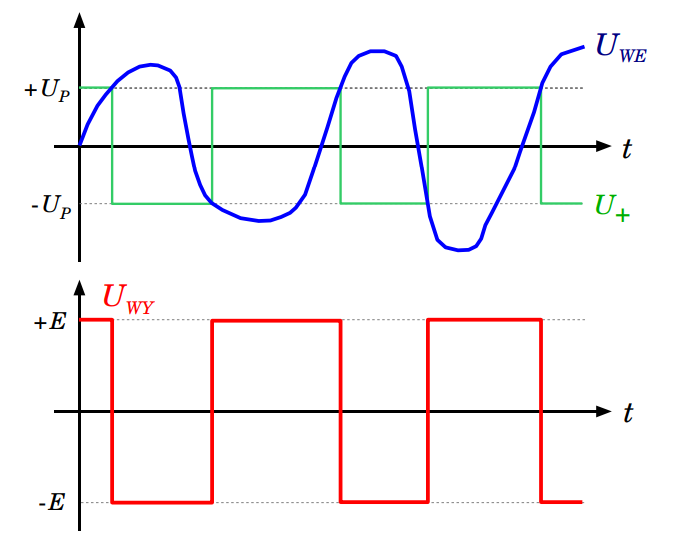
\includegraphics[scale=0.5]{img/theoretical/przerzutnik_reakcja.png}
            \caption{Teoretyczny przebieg}
            \label{fig:my_label}
        \end{figure}
    \item Zbudowany przerzutnik reaguje na zadane sygnały zgodnie z teoretycznymi przewidywaniami.
\end{itemize}

\pagebreak

\section{Histereza}

\begin{itemize}
    \item Do zmierzenia histerezy oraz wykreślenia statycznej charakterystyki układu należało włączyć \textbf{widok XY}.
    \item Teoretyczna pętla histerezy dla układu bistabilnego:
        \begin{figure}[H]
            \centering
            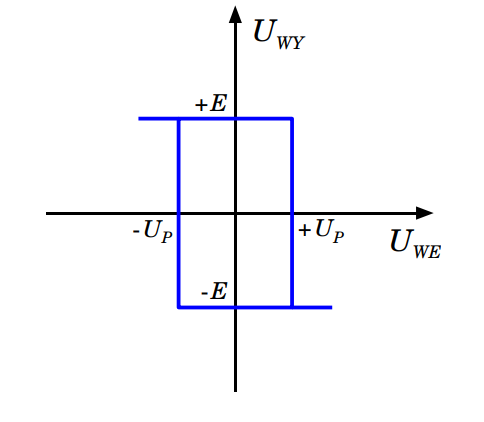
\includegraphics[scale=0.6]{img/theoretical/przerzutnik_histereza.png}
            \caption{Teoretyczna pętla histerezy}
            \label{fig:teoretyczna_histereza}
        \end{figure}
    \item Pętla histerezy wykreślona eksperymentalnie używając oporów (\ref{przerzutnik:R1}, \ref{przerzutnik:R2})
        \begin{figure}[H]
            \centering
            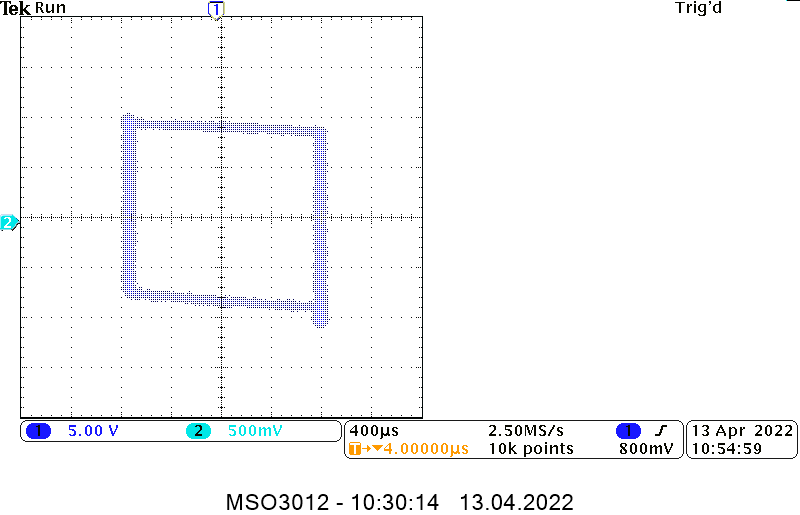
\includegraphics[scale=0.45]{img/osciloscope/1_4_histereza_XY_sin_cropped.png}
            \caption{Sygnał sinusoidalny na wejściu}
            \label{fig:histereza_sin}
        \end{figure}
        \begin{figure}[H]
            \centering
            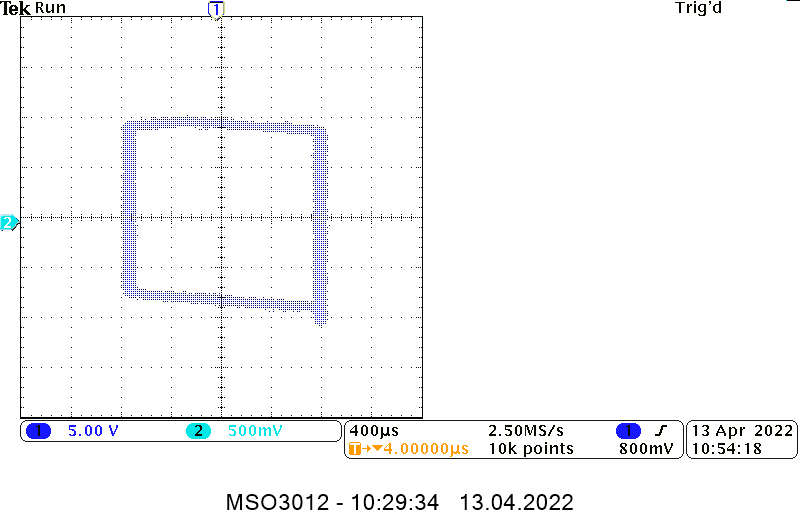
\includegraphics[scale=0.45]{img/osciloscope/1_4_histereza_XY_trojkat_cropped.png}
            \caption{Sygnał trójkątny na wejściu}
            \label{fig:histereza_sin}
        \end{figure}
    \item Teoretyczne wartości dla histerezy:
        \begin{center}
            +E = 11,96V (\ref{pomiar:U+})\\
            -E = -12.02V (\ref{pomiar:U-}) \\
            -$U_p$ = +$U_p$ = 1V 
        \end{center}
        Wartości +/-U = 1, ponieważ przeskok miał następować na 1V
    \item Wartości odczytane z histerezy:
        \begin{center}
            +E = -E $\approx$ 10V (2 odcinki na osi ze skalą równą 5V) \\
            -$U_p$ = +$U_p$ $\approx$ 1V (2 odcinki na osi ze skalą równą 500mV = 0.5V)
        \end{center}
    \item Eksperymentalnie wyznaczona histereza zgadza się z teoretyczną.
    \item Różnica między wartościami teoretycznymi a doświadczalnym mogą wynikać ze źle ustawionej skali bądź osi.
\end{itemize}